\section{Introduction}


In adversarial attacks, an attacker seeks to maliciously disrupt the performance of deep learning systems by adding small but often imperceptible noise to otherwise clean data~\citep{szegedy2013intriguing,goodfellow2014explaining}. Critical to the study of adversarial attacks is specifying the threat model~\cite{akhtar2018threat}, which outlines the adversarial capabilities of an attacker and the level of information available in crafting attacks. Canonical examples include the \textit{whitebox} threat model~\cite{madry2017towards}, where the attacker has complete access, and the less permissive \textit{blackbox} threat model where an attacker only has partial information, like the ability to query the target model \citep{chen2017zoo,ilyas2017query,papernot2016transferability}. 

Previously studied threat models (e.g., whitebox and blackbox) implicitly assume a static setting with full access to a target dataset~\citep{tramer2017ensemble}. However, such an assumption is unrealistic in many real-world systems. Countless real-world applications involve streaming data that arrive in an online fashion (e.g., financial markets or real-time sensor networks). Understanding the feasibility of adversarial attacks in this {\em online} setting is an essential question. 

As a motivating example, consider the case where the adversary launches a man-in-the-middle attack depicted in Fig.~\ref{fig:man_in_the_middle}. Here, data is streamed between two endpoints---i.e., from sensors on an autonomous car to the actual autonomous control system. 
An adversary, in this example, would intercept the streaming sensor data, potentially perturb it, and then send the corrupted data to the controller. Unlike classical adversarial attacks, such a scenario presents two key challenges that are representative of all online settings. 

\begin{wrapfigure}{o}{0.5\textwidth}
  %\begin{center}
    %\includegraphics[width=0.48\textwidth]{birds}
    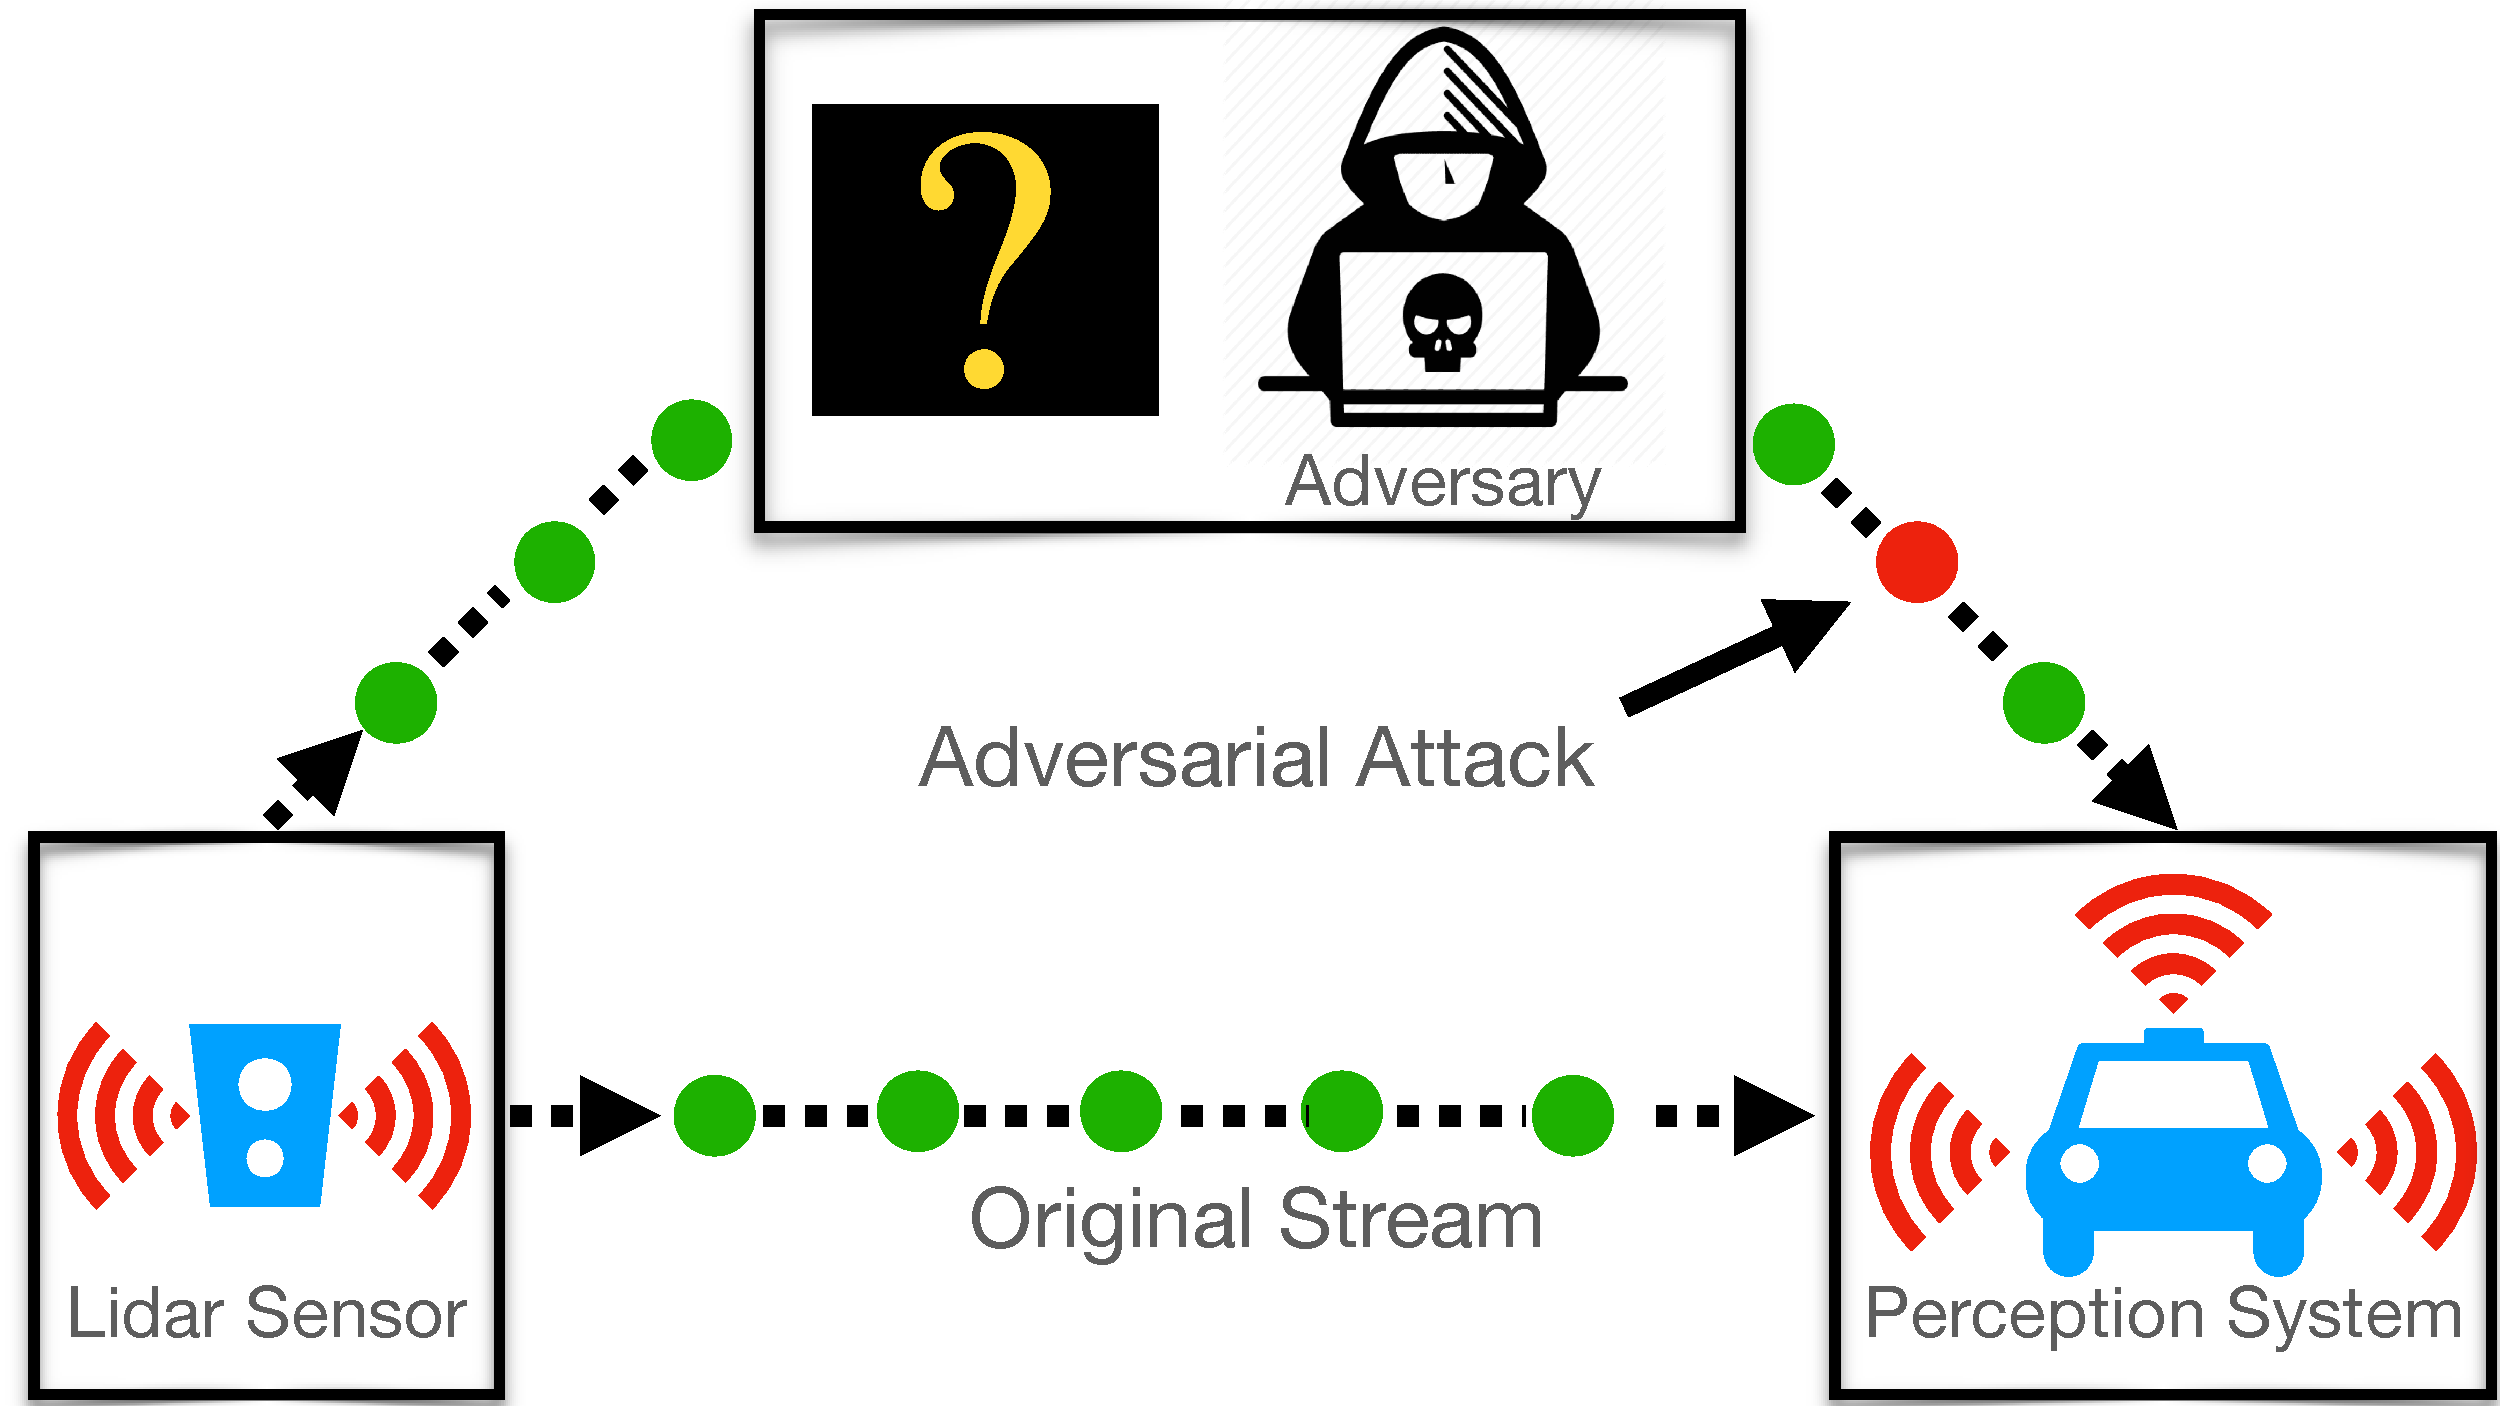
\includegraphics[width=0.48\textwidth]{Figures/man_in_the_middle_attack_2.pdf}
  %\end{center}
\caption{Man-in-the-Middle Attack.}
\label{fig:man_in_the_middle}
\end{wrapfigure}

\begin{enumerate}[noitemsep,topsep=0pt,parsep=0pt,partopsep=0pt, leftmargin=*] 
    \item \textbf{Transiency:} At every time step, the attacker must make an irrevocable decision on whether to attack the given datapoint. If the attacker fails, or opts not to attack, then that datapoint is no longer available for further attacks.
    \item \textbf{Online Attack Budget:} The adversary---to remain anonymous from stateful defences---is restricted to a small selection budget and must optimally balance a passive exploration phase before selecting high value items in the data stream (e.g. easiest to attack) to submit an attack on.
\end{enumerate}

To the best of our knowledge, the only existing approaches that craft adversarial examples on streaming data \citep{gong2019real,lin2017tactics,sun2020stealthy} require multiple passes through a data stream and thus cannot be applied in a realistic online setting where an adversary is forced into irrevocable decisions. Moreover, these approaches do not come with theoretical guarantees. Consequently, assessing the practicality of adversarial attacks---to better expose risks---in a truly online setting is still an open problem, and the central focus of this paper. Our main contributions are the proposal of a new \emph{online threat model} capturing the challenges of the online setting as well as providing a \emph{theoretical framework} (\S\ref{stochastic_k_secretary}) and a \emph{practical algorithm} (Alg.~\ref{alg:online_adv_attack}) to ground the study of online adversarial attacks. 


\xhdr{Main Contributions} 
We formalize an online threat model to study adversarial attacks on streaming data. In our online threat model, the adversary must execute $k$ successful attacks within $n$  streamed data points, where $k \ll n$. As a starting point for our analysis, we study the deterministic online threat model in which the actual value of an input---i.e., the likelihood of a successful attack---is revealed along with the input. Our first insight elucidates that such a threat model, modulo the attack strategy, equates to the $k$-secretary problem known in the field of optimal stopping theory \cite{dynkin1963optimum,kleinberg2005multiple}, allowing for the application of established online algorithms for picking optimal data points to attack. We then propose a novel online algorithm \algoname\ that is simple to implement for any pair $(k,n)$ and requires no additional hyperparameters, making it a natural choice for online adversarial attacks.
 

Besides, motivated by attacking blackbox target models, we also introduce a modified secretary problem dubbed the \textit{stochastic $k$-secretary problem}, which assumes the values an attacker observes are stochastic estimates of the actual value. We prove theoretical bounds on the competitive ratio for \emph{any} classical online algorithms in this setting. Guided by our theoretical results, we conduct a suite of experiments on both toy and standard datasets and classifiers (i.e., MNIST and CIFAR-10). Our empirical investigation reveal two counter-intuitive phenomena that are unique to the online blackbox transfer attack setting: 1.) In certain cases attacking robust models may infact be easier than non-robust models based on the distribution of values observed by an online algorithm. 2.) Simple attack strategies like FGSM can seemingly achieve higher online attack transfer rates than stronger PGD-attackers when paired with a online selection algorithm, demonstrating the importance of carefully selecting which data points to attack. Our key contributions are summarized as follows:

%We empirically show that even simple attack strategies can achieve high attack transfer rates when paired with an online algorithm, demonstrating the importance of carefully selecting which data points to attack.


\begin{itemize}[noitemsep,topsep=0pt,parsep=0pt,partopsep=0pt,label={\large\textbullet},leftmargin=*]
\item We formalize the online adversarial attack threat model as an online decision problem and rigorously connect it to a generalization of the k-secretary problem.
\item We introduce an online algorithm \algoname\ for the $k$-secretary problem and prove that it achieves a competitive ratio greater than $0.42737$ for $k=2$, outperforming the previous best single threshold algorithm \textsc{Single-Ref}~\cite{albers2020new}. 
\item We propose Alg.~\ref{alg:online_adv_attack} that leverages (secretary) online algorithms to perform efficient online adversarial attacks. We compare different online algorithms including \algoname\ via experiments on MNIST and CIFAR-10 in the challenging Non-Interactive BlackBox transfer setting.% and show that in many cases our onilne algorithm performs almost as well as an offline algorithm.
\end{itemize}

